\chapter{Introducción a la Energía Solar}
\label{solar}

\section{El Sol}
\label{elSol}
El Sol es tautológicamente la fuente de energía electromagnética más abundante y potente de nuestro sistema planetario. Nuestro planeta Tierra se ubica en la galaxia de la Vía Láctea en uno de sus brazos espirales llamado el brazo de Orión, en este brazo se encuentra un sistema llamado Solar\cite{solar:1}, sistema que lleva su nombre por su estrella principal, el Sol.\\

El Sol no solo pertenece a la historia moderna de la humanidad, en la literatura se encuentran infinidad de referencias y escritos dedicados a esta grandiosa estrella que ilumina nuestro planeta, es solo en la actualidad y en la historia reciente que esta estrella es referenciada como ''Sol'' pero para muchas culturas antiguas el Sol era una entidad muy importante, tanto así que para la cultura de la civilización egipcia representaba su deidad principal denominada Ra. En Latinoamérica se sabe que los incas le llamaban Inti, este era su principal deidad en la cual basaban todas sus costumbres, sistema de vida y ritos religiosos. Los griegos representaban al sol de manera un poco más compleja, como un carro arrastrado por 4 caballos el cual era conducido por Helios. Y así podríamos seguir mencionando multitud de referencias a la historia antigua en donde este astro era considerado uno de los dioses centrales y más importantes de la humanidad.\\ 

En astronomía el Sol está clasificado como una estrella del tipo espectral G2 y se encuentra ubicado en el centro del sistema solar. La luz emitida por el sol tarda 8 minutos y 19 segundos\cite{solar:2} en alcanzar el planeta Tierra y su energía constituye la fuente primordial del sustento de la vida basada en la fotosíntesis, es responsable del clima existente en nuestro planeta y de todas las condiciones de habitabilidad.\\

El sol se encuentra en una fase denominada secuencia principal, se formó aproximadamente hace 4.570 millones de años y se espera que continúe en la misma fase por otros 5.000 millos de años\cite{solar:4}.\\
Consecuencia de las reacciones termonucleares que se producen en el interior del sol, nuestro planeta recibe segundo a segundo cantidades muy grandes de energía. De manera sencilla, el Sol convierte cada segundo 564 millones de toneladas de Hidrógeno en 560 toneladas de Helio, esto quiere decir que aproximadamente 4 millones de toneladas de materia se convierten en energía que es expulsada al Universo, de la cual solo una pequeña porción es recibida por el planeta Tierra. En números, la energía producida por el sol se calcula aproximadamente en $3,8 x {10}^{23} [kWatts]$\cite{solar:3}\\

La radiación solar medida que inside en la atmósfera de nuestro planeta, alcanza los $1395 [W/{m}^{2}]$ este valor se denomina la \textbf{Constante Solar} y es un valor medio entre el valor máximo del \gloss{Perihelio} y el valor mínimo del \gloss{Afelio} (Ver Fig:\ref{afelioperielio}).\\

\begin{figure}[h!]
        \centering
        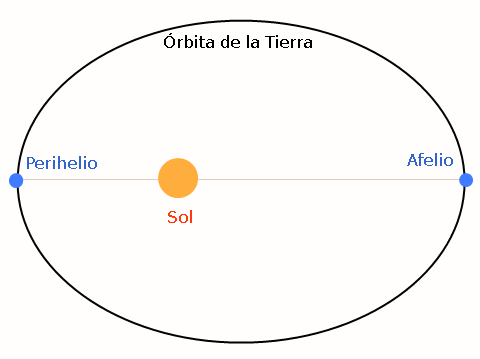
\includegraphics[scale=0.5]{images/afelioPerihelio}
        \caption{ Esquema que muestra la orbita de la Tierra con respecto al Sol y muestra los puntos del Afelio y el Perihelio}
	\label{afelioperielio}
\end{figure}

Como se mencionado, el Sol produce enormes cantidades de energía y ha sido venerado durante toda la historia de la humanidad y prácticamente cualquier referencia que se tiene de éste, apunta a cómo este astro permite que la vida se desarrolle en nuestro planeta, debido a todas estas características es que el hombre siempre ha intentado beneficiarse de la cantidad de energía que llega a nuestro planeta. Los intentos y logros han sido diferentes dependiendo de la época y los desarrollos tecnológicos de las civilizaciones, pero podríamos coincidir en que todas las civilizaciones antiguas y modernas han intentado producir energía a partir de su radiación, de alguna manera, todas lo han logrado, pero con diferentes niveles de eficiencia.\\

Para aprovechar esta energía, en la actualidad existen diversas tecnologías, entre las más usadas están la conversión a energía eléctrica, la conversión a energía térmica o el aprovechamiento del viento producido por el calentamiento de masas de aire, entre muchas otras. Cada tipo de conversión tiene diferentes niveles de eficiencia y en su aprovechamiento influyen muchos factores, dado el alcance de esta memoria nos enfocaremos en la conversión a energía eléctrica.\\

\begin{figure}[h!]
        \centering
        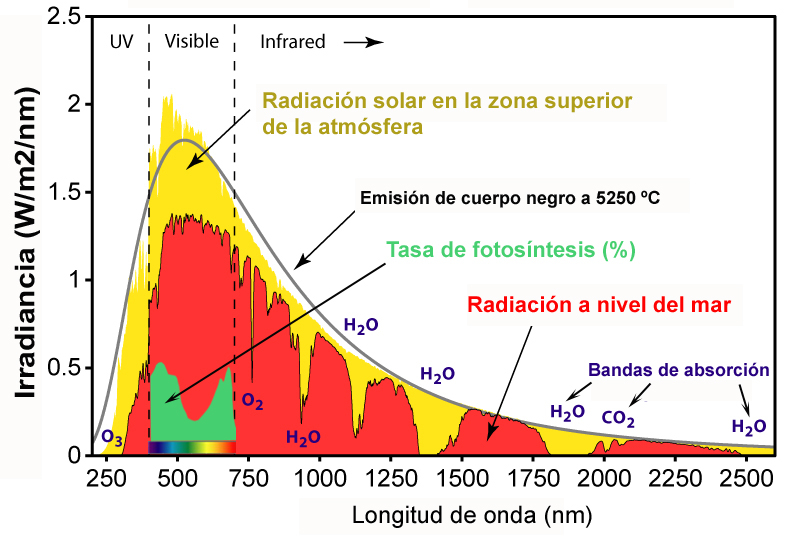
\includegraphics[scale=0.45]{images/espectroSolar}
        \caption{Gráfico de clasificación del espectro de la radiación solar\cite{recursoSolar:1}}
	\label{espectro}
\end{figure}

\section{La radiación solar}
La radiación emitida por el Sol viaja a través del espacio en forma de ondas electromagnética, como toda onda posee una longitud de onda y se puede clasificar de acuerdo a ésta. El espectro de la radiación solar se clasifica en tres grupos principales: la radiación UV, la luz visible y la radiación infrarroja (Ver. Fig. \ref{espectro}). Para los sistemas de producción de energía, el espectro que mas interesa es el espectro de radiación UV, que gracias a sus propiedades (longitud de ondas pequeñas) tienen la capacidad de excitar los átomos de silicio. Al contrario ocurre con el espectro infrarrojo que si bien aporta a la producción de energía, aporta mayoritariamente al aumento de temperatura de los paneles solares, lo que deriva en una disminución en su rendimiento.\\

Como se menciono en la sección \ref{elSol} la radiación capturada en la atmósfera es de $1395 [W/m^{2}]$, el problema que se presenta, es que la energía no puede ser captada desde el espacio para uso en la superficie terrestre, por lo tanto, la radiación proveniente del sol debe atravesar la atmósfera del planeta, la cual tiene un grosor aproximado de 80 km (ver Fig:\ref{fig:atmosfera}) y está compuesta de gases principalmente nitrógeno y oxígeno\cite{recursoSolar:1}. Al calentarse estos gases, producen, entre algunos fenómenos, los vientos que aportan a la formación de nubes, como consecuencia de esta absorción de energía en la atmósfera, incide una cantidad de energía bastante menor a la medida en el espacio cercano al planeta\\.

\begin{figure}[h!]
        \centering
        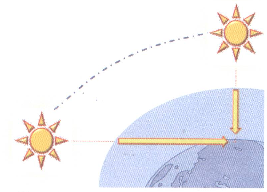
\includegraphics[width=240pt,height=160pt]{images/espesorAtmosfera}
        \caption{Distancia que atraviesa la radiación en la atmósfera}
	\label{fig:atmosfera}
\end{figure}
\newpage

Es debido a las condiciones climáticas y a la configuración química y física de la atmósfera que cada punto geográfico sobre la superficie terrestre recibirá diferentes cantidades de radiación.\\

Tal como mencionábamos con anterioridad, Chile presenta condiciones excepcionales en cuanto a la cantidad de radiación recibida en la superficie terrestre. Estudios realizados en nuestro país por diversas instituciones\cite{recursoSolar:2}, estiman que en el norte chileno es posible recibir más de 1000 $W/{m}^{2}$.\\

La radiación que inside sobre algún punto de la Tierra se denomina \gloss{gi}, esta radiación tiene 3 componentes: Radiación Directa Normal (\gloss{dni}), Radiación Difusa (\gloss{rd}) y Radiación Reflejada (ver Fig:\ref{fig:componentes}).
$$\fbox{GI = DNI + Rdifusa + Rreflejada}$$

\begin{figure}[h!]
        \centering
        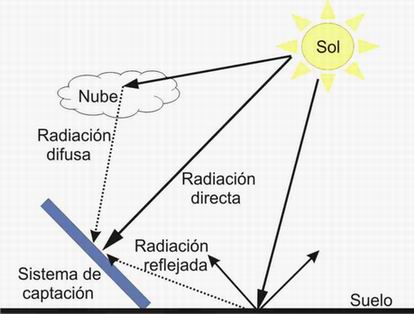
\includegraphics[scale=0.6]{images/radiacionDescompocicion}
        \caption{Descomposición de la radiación solar\cite{recursoSolar:1}}
	\label{fig:componentes}
\end{figure}

De esta definición derivan dos tipos de radiación que resultan relevantes para la producción energética fotovoltaica, la primera de ellas es la Radiación Global Horizontal (\gloss{ghi}) y la Radiación Directa Normal (\gloss{dni}). La \gloss{ghi} es la radiación medida en el plano horizontal a una superficie dada sobre la tierra, mientras que la \gloss{dni} es la radiación medida en dirección normal al Sol. Estas componentes se relacionan de la siguiente forma:
$$\fbox{GHI = DNI $\cos \theta$ + Rdifusa en plano horizontal+ Rreflejada}$$

\section{Energía Fotovoltaica}
Se llama luminosidad solar a la energía emitida por el Sol en un momento de tiempo dado, ahora bien es posible calcular la luminosidad que recibe la tierra en un momento puntual utilizando los valores de la constante solar definida en la sección \ref{elSol}. Esto se hace considerando que la luminosidad disminuye con la distancia entre el Sol, la Tierra y la superficie del planeta. Este calculo muestra que nuestro planeta recibe $3,65 x {10}^{23} [KW]$ de forma constante. Esta cantidad de energía es equivalente a 4.000 veces el consumo energético del planeta en una año.\\

Chile posee características naturales de excelencia en cuanto a la cantidad de radiación solar recibida desde el espacio (Ver. Fig. \ref{fig:mapaRadiacion}), estas condiciones posicionan a nuestro país dentro de la localidades con mejor componente solar en el planeta para la producción de energía fotovoltaica, a pesar de estas buenas condiciones nuestro país no ha desarrollado ni aplicado las tecnologías necesarias para aprovechar de buena manera esta ventaja.\\

\begin{figure}[h!]
        \centering
        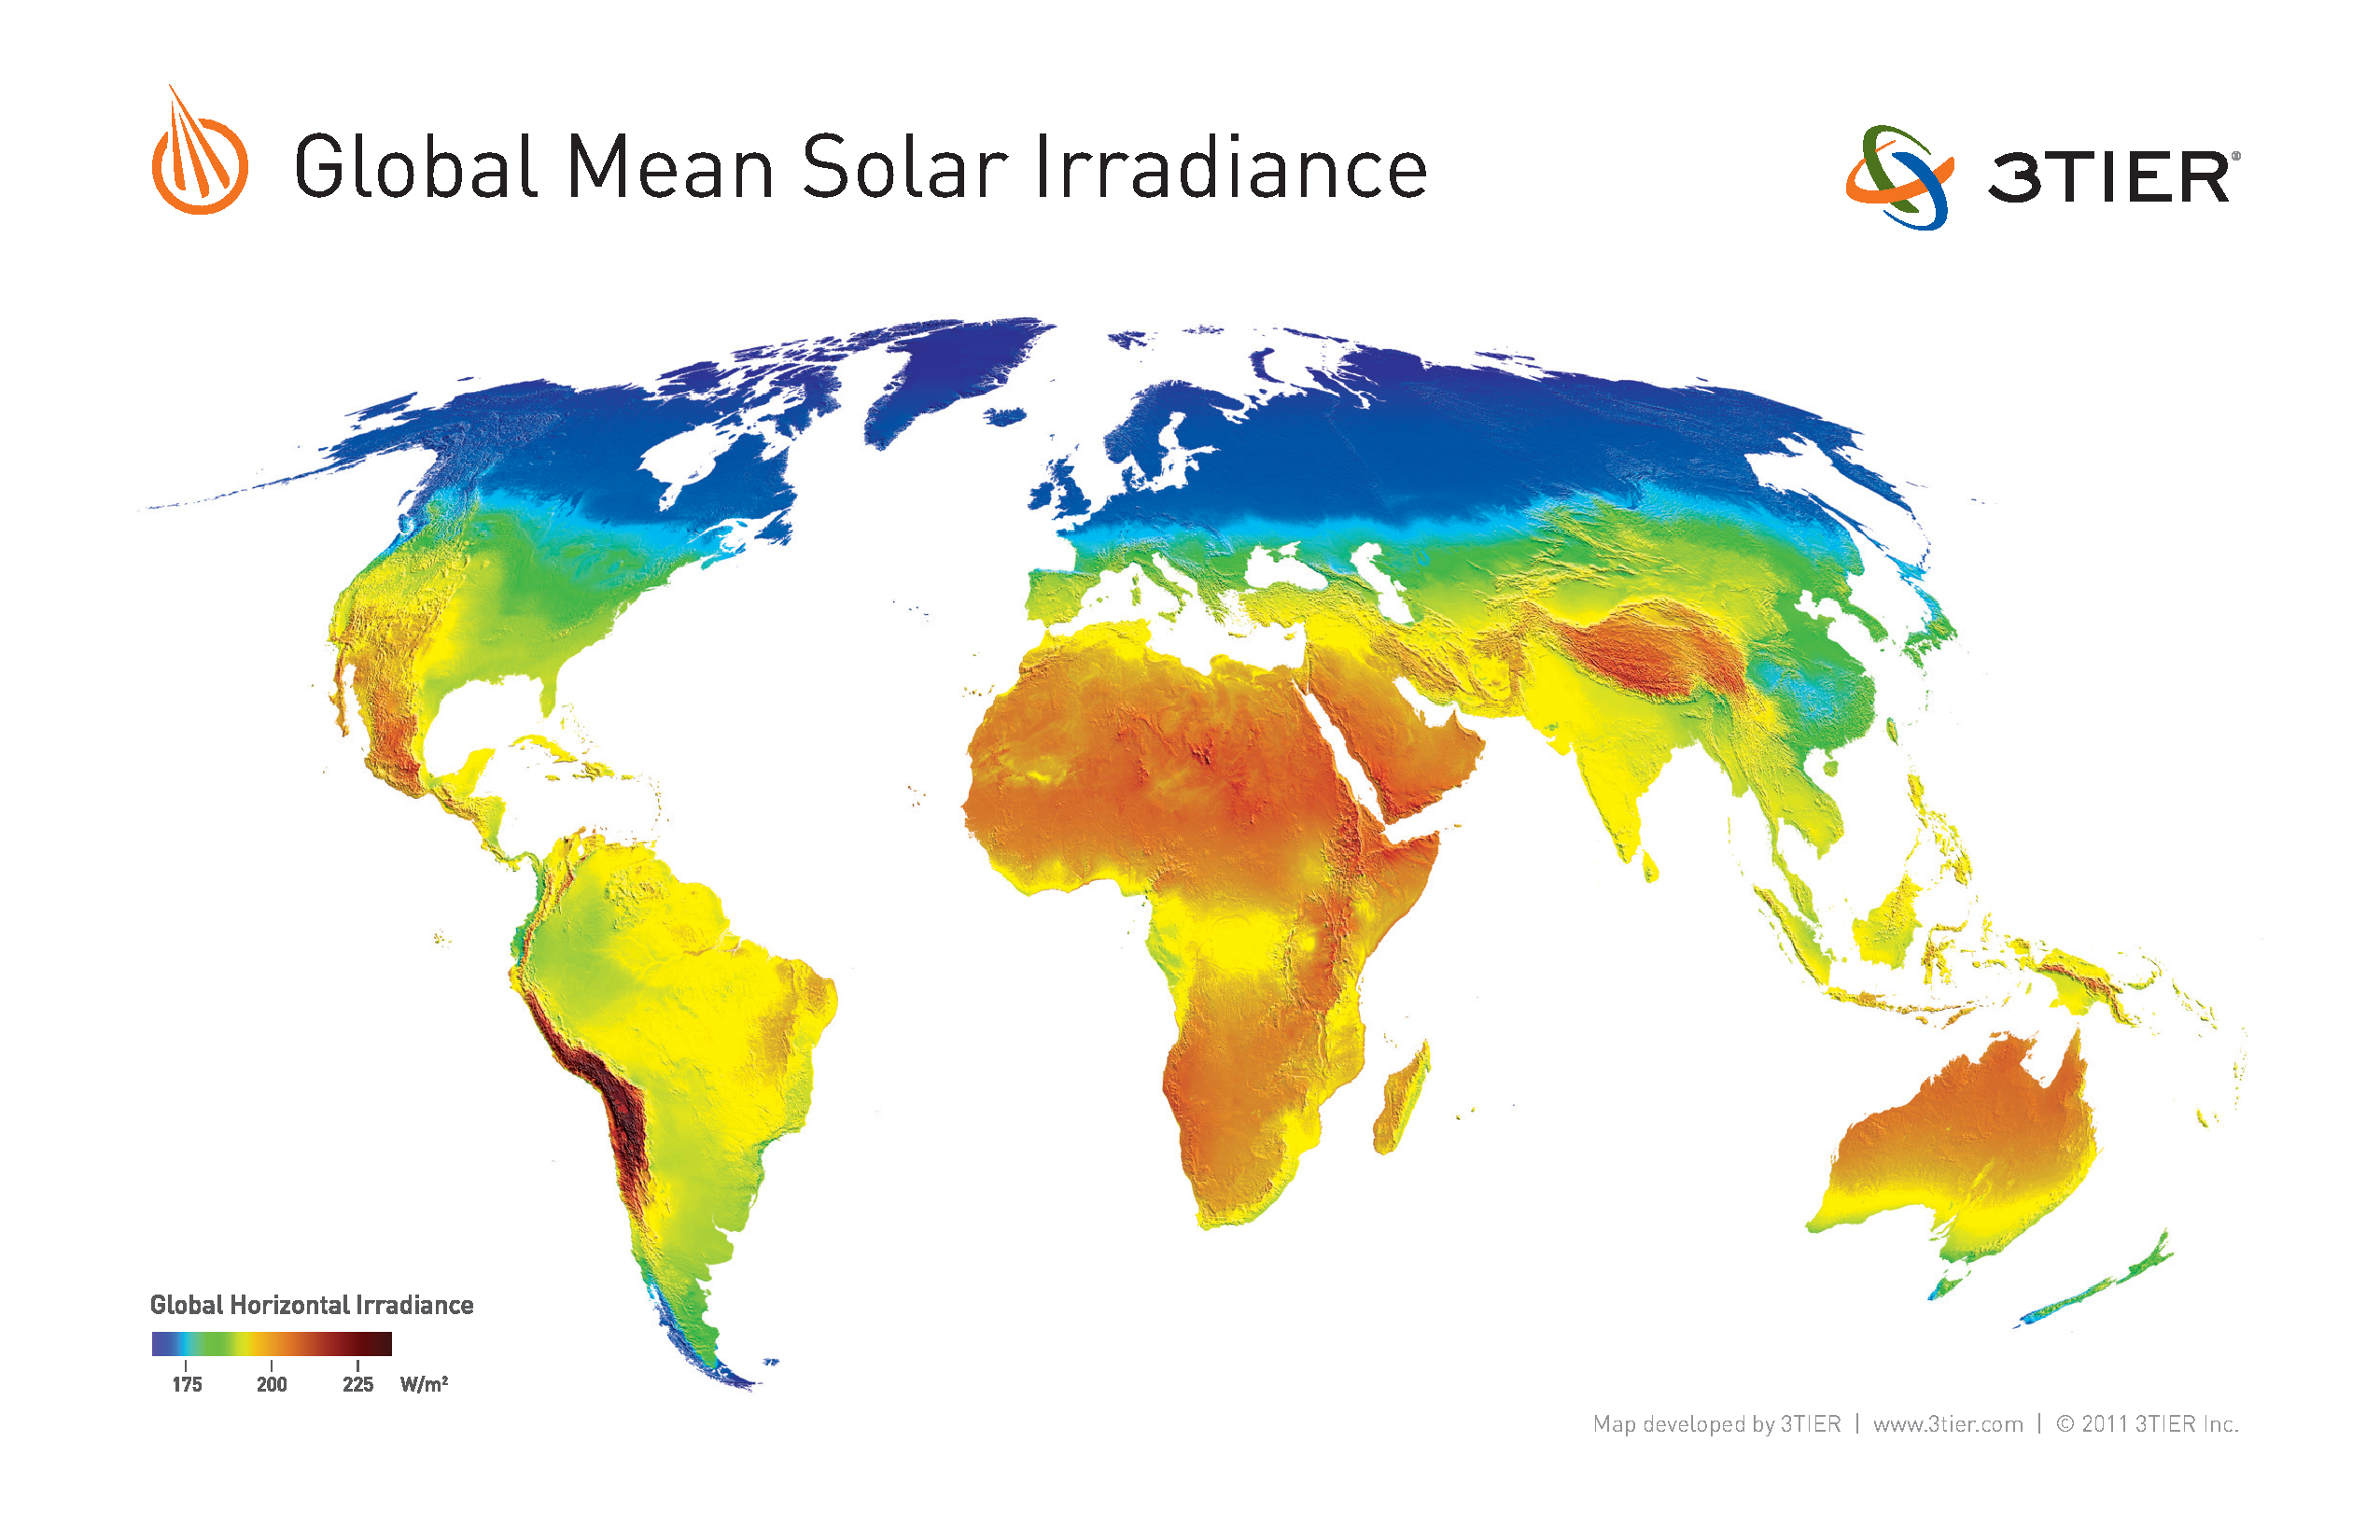
\includegraphics[scale=0.3]{images/3tier_solar_irradiance}
        \caption{Mapa de radiación solar mundial\cite{3tier}}
        \label{fig:mapaRadiacion}
\end{figure}

\newpage
La matriz energética de Chile tiene una potencia instalada de $15.548 MW$\cite{matrizEnergia:1}, de la cual el 63\% es energía termoeléctrica, un 34\% es energía hidroeléctrica y 3\% corresponde a energía eólica. Del 63\% de energía termoeléctrica, se considera la producida por el gas natural, el carbón y el petróleo. Adicionalmente, de toda la matriz, el 75\% es importada, esto quiere decir que nuestro país al año 2011 es incapaz de autoabastecerse enérgicamente, depende de la cantidad de energía que esté disponible para la venta desde el exterior, esto suena contradictorio considerando que Chile tiene los mejores recursos solares del mundo.\\
Para graficar de forma sencilla la capacidad solar de Chile podemos hacer algunos cálculos sencillos.\\ La CNE dice que al año 2010 chile consume $58.257 GWh$, considerando condiciones climáticas relativamente buenas\footfullcite{foot:datoCalama} en el norte del del país tenemos:$$\fbox{58.257.000 [MWh] / 0,255 [MWh/$m^2$] = 228.458.823 $m^2$}$$
 
Ahora bien esta cifra es solo referencial al potencial que chile posee para producir energía, ciertamente que detrás de toda instalación de este tipo hay otras consideraciones ambientales que tomar en cuanta, por ejemplo, el impacto ambiental a causa de la extensa área de paneles a instalar. Por otro lado, un sistema distribuido con pequeñas centrales a lo largo de todo el país, ayudaría a disminuir el impacto en comparación a un sistema centralizado junto a una gran linea de transmisión.

En Chile existen importantes experiencias, en investigación y aplicación, donde Chile ha sido pionero\cite{colegioIng:2}, a pesar de esto han sido otros países especialmente europeos quienes han recogido estas investigaciones y han potenciado el desarrollo de esta tecnología, países como España y Alemania hoy en día lideran la producción e investigación en energías renovables no convencionales.\\

\section{Sistemas fotovoltaicos}
Para capturar la radiación solar incidente en la superficie terrestre y transformarla a energía eléctrica se debe utilizar un conjunto de componentes de hardware eléctricos, el sistema más básico consta de un panel solar, un inversor y una batería. Uno de los grandes problemas del sector energético ha sido durante mucho tiempo el cómo se debe almacenar la energía producida y los sistemas fotovoltaicos no están ajenos a este problema, principalmente porque la radiación solar no es constante durante el día ni mucho menos durante el año, más aún un sistema fotovoltaico sólo producirá energía eléctrica durante las horas de sol o mientras los fotones de las ondas electromagnéticas provenientes del sol exciten los átomos de silicio. En términos técnicos, una instalación solar tiene un factor de planta muy bajo en comparación a otras instalaciones (termoeléctricas o hidroeléctricas).\\

Las primeras referencias que se tienen de paneles solares son del año 1954 cuando se descubrió que el silicio con ciertas impurezas era muy sensible a la luz. Uno de los datos interesantes aquí es que el silicio es el segundo elemento más abundante en la Tierra después del oxígeno con un 28\% de la masa total.

Los primero paneles solares que se fabricaron, sólo tenían una eficiencia el 4.5\%, sin embargo fue durante la segunda mitad de la década del 1950 cuando esta tecnología empezó a desarrollarse con más fuerza debido a la carrera espacial entre EEUU y la Unión Soviética durante 1950 y 1980.\\

Los paneles solares están fabricados por una gran cantidad de pequeñas celdas hechas de silicio, además de otros materiales como aluminio y cobre en menor proporción. El silicio utilizado en la confección de dichas celdas, se extrae de la corteza terrestre, el problema es que no se encuentra en su forma pura y es necesario someterlo a diferentes procesos químicos para purificarlo. Durante mucho tiempo este proceso fue de costos muy elevados, pero en la actualidad la tendencia es a reducirse de manera significativa gracias al desarrollo de la tecnología y a la masificación de las ERNC. A pesar de esto la energía requerida para purificar el silicio para la formación de paneles es bastante alta y un panel debe funcionar por algunos años antes de recuperar la energía utilizada en su confección. Esto se contrasta gracias a que la vida útil de un panel puede llegar a ser de 30 a 40 años, sin requerir mantención.\\

Un sistema fotovoltaico adicionalmente requiere de otro componente eléctrico para operar, el inversor, este componente es el encargado de convertir la corriente DC (producida por los paneles) en corriente AC, que es el tipo de corriente con la cual operan prácticamente todos lo componentes eléctricos actuales y es el tipo de corriente que se usa para ser transmitida a diferentes puntos geográficos del país.\\

Finalmente si el sistema es un sistema aislado de los ''sistemas interconectados'' se suele utilizar algún tipo de batería o almacenador de energía para suplir la demanda en horas donde el sistema no puede producir energía. Si el sistema esta conectado a ''la red'' la demanda se compensa con la energía aportada por la red y la sobre producción se inyecta a esta para que pueda ser utilizada por otros usuarios. A la fecha de publicación de este documento, en el congreso Chileno se discute la ley que permitirá a pequeños productores de energías renovables vender la sobreproducción a sistema interconectado.

